% !TEX root = ../main.tex

%************************************************
\chapter{Introduction}
\label{ch:intro}
%************************************************

In 1963, the powerful radio source 3C 273 was identified with a star-like, thirteenth magnitude object with a strongly redshifted ($z=0.158$) \marginpar{$z=\frac{\Delta \lambda}{\lambda_0}$} optical spectrum \citep{schmidt63}. 
Assuming this redshift was due to the Hubble expansion of the Universe, 3C 273 was at an enormous distance (500 megaparsecs) and was 10 times optically brighter than the most luminous galaxies. 
Variability on time-scales of weeks suggested that the source was very compact.
It was quickly realised that quasars, and other lower-luminosity classes of active galactic nuclei (AGN)\footnote{Throughout this thesis we use the terms `quasar' and `Active Galactic Nucleus (AGN)' interchangeably to describe active super-massive black holes, although the term quasar is generally reserved for the luminous (L$_{\rm Bol} > 10^{12}{\rm L}_{\odot}$) subset of AGNs.}, are powered by the release of gravitational potential energy as mass is accreted onto a super-massive \marginpar{Super-massive: $10^{6 - 9}$ M$_\odot$} black hole (BH) at the centre of a galaxy \citep[e.g.][]{hoyle63,salpeter64,lynden-bell69,lynden-bell71}. 

Begining in the early 1990s, inactive super-massive BHs were found in the centres of many nearby massive galaxies \citep[e.g.][]{kormendy95,ferrarese05,kormendy13}.
This proved that, rather than being exceptional galaxies which happen to harbour BHs, quasar activity was in fact a stage in the life of all massive galaxies \citep[e.g.][]{lynden-bell69}. 
Shortly after, it was discovered that the BH mass and the properties of the host-galaxy bulge were strongly correlated \citep[e.g. the M$_{\rm BH}$-$\sigma$ relation][]{ferrarese00,gebhardt00,graham01,tremaine02,marconi03,aller07,gultekin09}. \marginpar{$\sigma$: stellar velocity dispersion of host galaxy spheroid/bulge}
This was an unexpected finding, given that the sphere-of-influence \marginpar{Sphere-of-influence: where the gravity of the BH dominates over the other mass components (stars, gas etc.)} of a BH is many orders of magnitude smaller than the size of a galactic bulge. 
It suggested that the BH and the bulge grow synchronously, with the energetic output of the rapidly-accreting BH coupling with the gas in the host galaxy and regulating star formation and the growth of the BH itself \citep[e.g.][]{silk98,king03,dimatteo05,king15}. 

The number density of quasars, which evolves strongly with redshift, peaks at redshifts $2 \lesssim z \lesssim 3$ \citep[e.g.][]{brandt05,richards06b} and the most massive (M$_{\rm BH} \gtrsim 10^9\msun$) present-day BHs experienced much of their growth during this epoch.  
The cosmic star formation rate history closely follows the cosmological evolution of the quasar luminosity function \citep[e.g.][]{boyle98}, which establishes a further connection between BH and galaxy properties.
Quasar feedback has also been invoked to reproduce the high-mass end of the galaxy luminosity function in cosmological simulations \citep[e.g.][]{kauffmann00}.
The insight that quasars could play a crucial role in the evolution of galaxies has led to an explosion of interest in their properties. 

\section{AGN: current paradigm}

\begin{figure}
  \centering
  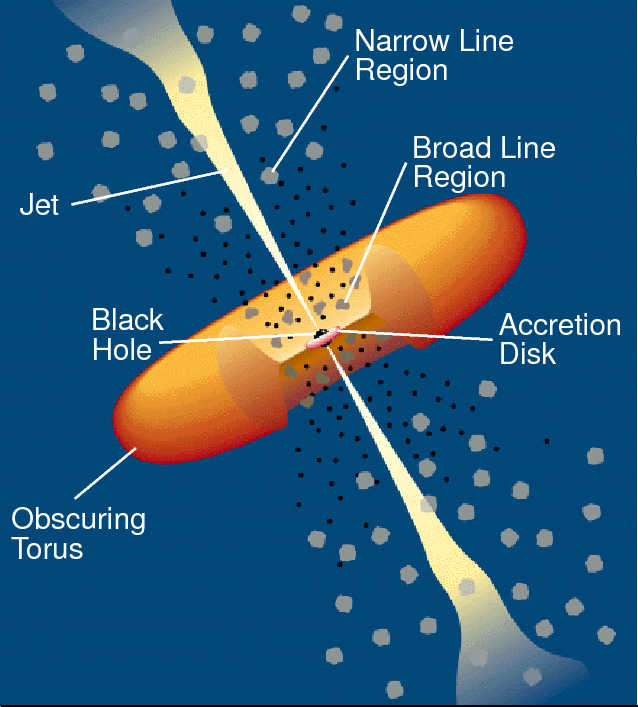
\includegraphics[width=0.5\textwidth]{figures/chapter05/urry_model}
  \caption[{Illustration of the physical structure of an AGN in a simple orientation-based unification model.}]{Illustration of the physical structure of an AGN in a simple orientation-based unification model. Figure taken from \citet{urry95}.}
  \label{fig:agnmodel}
\end{figure}

The current AGN paradigm is widely accepted, although many of the details are unknown. 
The basic features are: a hot accretion disc surrounding a super-massive BH, rapidly orbiting clouds of ionised gas, and a dusty, obscuring structure (generally referred to as the `torus'). 
Collimated jets of relativistic plasma and/or associated lobes are also seen in the 10 per cent of quasars that are radio-loud \citep[e.g.][]{peterson97}. 
The cartoon picture illustrating the basic structure of an AGN is shown in Figure~\ref{fig:agnmodel}. 

\subsection{Accretion disc}

Material is pulled towards a super-massive BH and sheds angular momentum through viscous and turbulent processes in a hot accretion disc \citep[e.g.][]{begelman85}. 
The accretion disc reaches temperatures of $\sim$$10^6$K, and radiates primarily at ultraviolet (UV) to soft-X-ray wavelengths. 

\subsection{The broad line region}

One of the pre-eminent features of many AGN spectra are broad optical and UV emission lines produced in the broad line region (BLR). 
The BLR consists of gas clouds at distances from several light-days to several light-months that are photo-ionised by the ultraviolet continuum emission emanating from the accretion disc.  
Because of the close proximity to the central super-massive BH, bulk motions are dominated by gravity and radiation pressure from the accretion disc.
The very broad emission line widths are assumed to Doppler-broadened, and imply line-of-sight velocities of many thousands of \kms. 

\subsection{The dusty torus}

Further out are dusty, molecular clouds which are co-planar with the accretion disc. 
These dusty clouds are generally referred to as the `torus'. 
In a Type II AGN, the accretion disc is observed in an edge-on configuration and, as a result, emission from the accretion and BLR is obscured by the dusty torus \citep[e.g.][]{antonucci93}.
Although this simple picture (shown in Figure~\ref{fig:agnmodel} as well as in countless other publications) is a useful staring point, the idea of a torus as a static, doughnut-like structure is almost certainly incorrect. 
For example, the problem of maintaining the large scale height required by unification schemes has long been recognized. 
In one alternative scenario, the torus is the dusty part of an accretion disc wind that extends beyond the dust-sublimation radius \citep[e.g.][]{konigl94,everett09,gallagher12,everett05,keating12,elitzur06}. 

\subsection{The narrow line region}

Further away from the central BH and beyond the dusty torus is the narrow emission line region (NLR). 
Like the BLR, the NLR is ionised by radiation from the central source. 
Unlike the BLR, densities in the NLR are low enough that forbidden transitions are not collisionally suppressed. 
Emission line widths are typically hundreds of \kms in the NLR. 
The NLR is sufficiently extended to be spatially resolved. 
\todo{Extent: ask Paul/Manda}

\section{Winds and outflows in AGN}

Quasars are very powerful sources of radiation, and are embedded in matter-rich environments at the centres of galaxies.
Strong winds, driven by some combination of gas pressure, radiation pressure, and magnetic forces, are to be expected under these conditions \citep[e.g.][]{blandford82b,proga00,everett05}. 
In line with these expectations, evidence for outflows is common in the spectra of quasars. 

Perhaps the most dramatic evidence of outflows is seen in broad absorption line quasars \citep[BALQSOs;][]{weymann91}.
BALQSOs are characterised by broad absorption features in the ultra-violet resonance lines of highly ionised \ion{N}{V}, \ion{C}{IV} and \ion{Si}{IV}. 
The absorption is always blueshifted, and is evidence for fast outflows with velocities as large as 60\,000 \kms \citep[e.g.][]{turnshek88}. 
The observed \ion{C}{IV} BALQSO fraction in radio-quiet quasars is $\sim$$15$ per cent \citep[e.g.][]{hewett03,reichard03} and the intrinsic fraction in the quasar population has been estimated at $\sim$$40$ per cent \citep{allen11}.
Outflows are also used to explain narrow UV and X-ray absorption lines (NALs) which are seen in $\sim$$60$ per cent of Seyfert 1 galaxies \citep{crenshaw99} and some quasars \citep[e.g.][]{hamann97}. 

The blueshifting of high-ionisation lines in the BLR (including \ion{C}{IV}) can be understood if the lines are produced in outflowing clouds, with the accretion disc blocking our view of the receeding clouds on the far side (although see Gaskell for an alternative explanation). 
The blueshifting of \ion{C}{IV} appears to be nearly ubiquitous in the quasar population \citep[e.g.][]{richards02,richards11}, suggesting that outflows are very common in the vicinity of quasars. 

Accretion-disc wind models have been developed to explain the wide range of emission and absorption line phenomena described above \citep[e.g.][]{murray95,elvis00,proga00,everett05}.
UV photons excite the partially-ionised material surrounding the accretion disc. 
This exerts a pressure on the atoms - a phonemonon known as radiation line-driving - and a wind is blown from the accretion disc. 

Observations of blueshifted absorption and emission lines suggest that the energy released by quasars can have a dramatic effect on their immediate surroundings.  
However, can the energy quasars release have an impact on galactic scales? 

In recent years, a huge amount of resources have been devoted to searching for observational evidence of galaxy-wide, quasar-driven outflows \citep[for recent reviews, see][]{alexander12,fabian12,heckman14}. 
This has resulted in recent detections of outflows in AGN-host galaxies using tracers of atomic, molecular, and ionised gas with enough power to sweep their host galaxies clear of gas \citep[e.g.][]{nesvadba06,arav08,nesvadba08,moe09,dunn10,alexander10,harrison12,harrison14,nesvadba10,rupke13,veilleux13,nardini15,feruglio10,alatalo11,cimatti13,cicone14}.  
However, despite considerable observational and theoretical support for a `feedback' relationship, any underlying causal mechanism(s) responsible for the M$_{\rm BH}$-$\sigma$ relation is yet to be conclusively identified. 

\section{Measuring black hole masses}

The BH mass is one of the most important physical parameters of a quasar. 
Quantifying the growth-rate of massive BHs at $2 \lesssim z \lesssim 3$ is crucially important in understanding the role quasars play in galaxy evolution.
For example, the processes responsible for the M$_{\rm BH}$-$\sigma$ relation can be understood by measuring the evolution of this relation over time \citep[e.g.][]{bennert11}. 
Quasar-driven outflows are thought to play a critical role in forging the M$_{\rm BH}$-$\sigma$, and the power of these outflows is directly proportional to the BH mass. 
The distribution of quasars in the BH mass-quasar luminosity plane also conveys important information about the accretion processes occuring in active BHs \citep[e.g.][]{kollmeier06}.
Considerable resources have therefore been devoted to developing methods of measuring BH masses, and these are now described. 
The focus of this thesis is on the virial method, which is calibrated using results from reverberation-mapping. 
At present, this is the only method for deriving BH masses for large numbers of objects at high-redshifts, which is needed to understand quasar feedback. 

The mass of a BH, or indeed any object, can be measured from the velocity and characteristic scale of test particles in orbit around it. 

\subsection{Dynamical modelling}

The masses of BHs in many local, inactive galaxies have been measured by dynamical modelling spatially resolved kinematics of gas and stars. 
However, this requires the sphere-of-influence of the BH, $R_{\rm BH}$, to be resolved. 
With BH masses only $\sim$0.1 per cent of the stellar mass of the host galaxies, $R_{\rm BH}\sim1-100$ parsec \citep{kormendy13}.
With current instrumentation, resolving this region is only possible in very close by galaxies. 

\subsection{Reverberation mapping}

Under the assumptions that the BLR dynamics are virialised \marginpar{The virial theorem states...} and the gravitational potential is dominated by the BH, the BH mass is given by:

\begin{equation}
M_{\rm BH} = \left( \frac{V_{\rm Virial}^2R}{G} \right)
\end{equation}

where $V_{\rm virial}$ is the virial velocity in the BLR and $R$ the characteristic BLR radius.
Under the virial assumption, the problem of measuring the mass therefore reduces to the problem of measuring the velocity and radius of the line-emitting clouds in the BLR. 

Continuum variability is a common characteristic of quasars, owing to the stochastic nature of the accretion process.  
Because the BLR is photo-ionized by the continuum, the broad emission lines also vary with some characteristic lag, which is related to the light travel time across the BLR. 
The reverberation mapping method, first proposed by \citet{blandford82a}, uses the time lag between variations in the continuum emission and correlated variations in the broad line emission to measure the typical size of the BLR \citep[e.g.][]{peterson93,netzer97,peterson14}. 

The typical velocity in the BLR is measured from the Doppler-broadened width of an emission line produced in the BLR. 
Since the structure and geometry of the BLR is unknown, a virial coefficient $f$ is introduced to transform the observed line-of-sight velocity inferred from the line width in to a virial velocity.
This introduces a significant uncertainty into the mass estimates, because $f$ is unknown and likely varies from object to object.  
In practice, the value of $f$ is empirically determined by requiring that the derived masses are consistent with those predicted from the M$_{\rm BH}$-$\sigma$ velocity dispersion of galaxy} relation for local inactive galaxies. 

Because reverberation mapping depends on temporal resolution rather than spatial resolution, this technique can be applied out to much greater distances than direct dynamical modelling.
However, because reverberation mapping relies on dense spectrophotometric monitoring campaigns which span many years, lags have been measured for only $\sim50$ AGN \citep[e.g.][]{kaspi00,peterson04,kaspi07,bentz09,denney10,barth11,grier12}. 
This sample is strongly biased to low luminosity Seyfert 1 galaxies \marginpar{Seyfert 1:}, and the maximum redshift is just $z\sim0.3$. 
Comprehensive statistical studies of active BHs, particularly during the epoch of peak galaxy formation ($z\gtrsim2$, require a different approach. 

\subsection{Single-epoch virial estimates}

Reverberation mapping campaigns have also revealed a tight relationship between the radius of the BLR and the quasar optical (or ultraviolet) luminosity \citep[the $R-L$ relation; e.g.][]{kaspi00,kaspi07}.
A slope of $\simeq0.5$ is found, which consistent with the naive prediction \citep[e.g.][]{peterson97}. 
An advantage of the technique is that it is inexpensive in telescope time. 
A single spectrum yields a mass measurement. 
This relation provides a much less expensive method of measuring the BLR radius, and large-scale studies of AGN and quasar demographics have thus become possible through the calibration of single-epoch virial-mass estimators using the reverberation-derived BH masses \citep[e.g.][]{greene05b,vestergaard06,vestergaard09,shen11,shen12,trakhtenbrot12}.
Single-epoch virial BH mass estimates normally take the form

\begin{equation}
  \label{eq:virialmass}
  \mathrm{M_{BH}} = 10^{a} \left( \frac{\Delta V}{1000~\mathrm{km~s^{-1}}} \right)^b \left[ \frac{L_{\lambda}}{10^{44}~\mathrm{erg~s^{-1}}} \right]^c
\end{equation}

\noindent where $\Delta V$ is a measure of the line width (from either the FWHM or dispersion), $L_\lambda$ is the monochromatic continuum luminosity at wavelength $\lambda$, and $a$, $b$, and $c$ are coefficients, determined via calibration against a sample of AGN with reverberation-mapping BH mass estimates. Several calibrations have been derived using different lines (e.g. \hbns, \ion{Mg}{II}, \ion{C}{IV}) and different measures of the line width (FWHM or dispersion) \citep[e.g.][]{vestergaard02,mclure02,vestergaard06,mcgill08,wang09,rafiee11,park13}.

The uncertainties in reverberation mapped BH masses are estimated to be $\sim 0.4$ dex \citep[e.g.][]{peterson10}, and the uncertainties in virial masses are similar \citep[e.g.][]{vestergaard06}.

Furthermore, if the BLR is anisotropic \citep[for example, in a flattened disk; e.g.][]{jarvis06} then the line width will be orientation-dependent \citep[e.g.][]{runnoe13b,shen14,brotherton15}. 

The main progress in this area in recent years, that enables comprehensive statistical studies of active black holes (BHs), is the success of the large reverberation mapping project. 
This allows reliable estimates of broad line region (BLR) sizes and BH masses. 
The main concern and the biggest unknown is the extension of the method to high redshifts where \hb measurements are no longer available. 
Something we will explore in Chapter~\ref{ch:bhmass}. 

We emphasize that application of single-epoch spectroscopy to quasars rests on the untested assumption that machinery which is calibrated for sub-Eddington BHs with M$\sim10^7$ still works for BHs with masses up to $10^{10}$ that radiate near the Eddington limit. 
Refer forward to problems with \ion{C}{IV} (Chapter 3)

For example, single epoch estimates have been used to calculate black hole masses in the highest redshift quasars to study the growth of SMBHs. 
This figure shows a compilation of SE mass estimates for quasars over a wide redshift range from different studies. 
These studies show that massive, $10^9$ BHs are probably already in place by $z\sim7$, when the age of the Universe is less than 1 Gyr.
The fact that a SMBH exists in a quasar at such high redshift is of great importance in physics.
The high redshift means that it was already there when our universe was very young, only about
800 million years old. And the fact that a SMBH was able to grow up in such a short time put
some very tight constraints upon both the cosmological parameters and the accretion history of the
SMBH itself (Willott et al. 2003).
Clustering (Shen \& Ho 2014; Timins et al.?). 

Quasar black hole masses: \citet{shen13}, \citet{peterson10}, \citet{peterson11}, \citet{vestergaard11}, \citet{marziani12}. 


The vast majority of reverberation-mapping lag measurements have been done using \hbns, and the $R-L$ relation has been established using \hbns. 
Almost all of these use the broad \hb emission-line.
The full width at half maximum (FWHM) or dispersion ($\sigma$; derived from the second moment) velocity of the prominent broad emission line of \hb (4862.7\AA) is used as an indicator of the virial velocity, with extensions to other low-ionization emission lines such as \ha (6564.6\AA) and \ion{Mg}{II}\ll2796.4,2803.5 \citep[e.g.][]{vestergaard02,mclure02,wu04,kollmeier06,onken08,wang09,rafiee11}.
\marginpar{FWHM: Full width of the line profile at half of maximum intensity}



\section{Lots of data is now available}

Palomar-Green (PG) Bright Quasar Survey (BQS; Schmidt \& Green 1983), the first large-area quasar survey, identificed 114 quasars via their UV excess. 
Boroson \& Green (1992) were among the first to analyse quasar spectroscopic properties in a systematic way.

With the advent of CCD technology came a new generation of surveys, most notably the Sloan Digital Sky Survey (SDSS). 
SDSS, and the next generation Baryon Oscillation Spectroscopic Survey (BOSS), now contain spectra of $\sim200\,000$ quasars. 

AGN emit strongly over many decades in frequency of the electromagnetic frequency. 
This makes studying them a challenge. 
However, we are also able to take advantage of a number of recent, sensitive, wide-field photometric surveys, including SDSS (in the UV/optical), UKIDSS (in the NIR) and WISE (in the mid-infrared) providing good multi-wavelength coverage and large dynamic range in luminosity and redshift.  

\section{Overview of thesis}

\subsection{Chapter 1: A near-infrared spectroscopic database of high-redshift quasars}

With spectra from SDSS we can derive BH masses and outflow properties from optical lines. 
But these are shifted to infrared wavelengths at redshifts > 1, when things get interesting. 
Increasing availability of near-infrared spectra. 

\subsection{Chapter 2: Black Hole Masses}

Black-hole masses are crucial to understanding the physics of the connection between quasars and their host galaxies and measuring cosmic black hole-growth. 
At high redshift, $z \gtrsim 2.1$, black hole masses are normally derived using the velocity-width of the \ion{C}{IV}\ll1548,1550 broad emission line, based on the assumption that the observed velocity-widths arise from virial-induced motions.  
In many quasars, the \ion{C}{IV}-emission line exhibits significant blue asymmetries (`blueshifts') with the line centroid displaced by up to thousands of \kms\, to the blue. 
These blueshifts almost certainly signal the presence of strong outflows, most likely originating in a disc wind.
We have obtained near-infrared spectra, including the \ha\l6565 emission line, for 19 luminous ($L_{\rm Bol} = 46.5-47.5$ erg~s$^{-1}$) Sloan Digital Sky Survey quasars, at redshifts $2 < z < 2.7$, with \ion{C}{IV} emission lines spanning the full-range of blueshifts present in the population.  
A strong correlation between \ion{C}{IV}-velocity width and blueshift is found and, at large blueshifts, $>$2000\,\kms, the velocity-widths appear to be dominated by non-virial motions. 
Black-hole masses, based on the full width at half maximum of the \ion{C}{IV}-emission line, can be overestimated by a factor of five at large blueshifts. 
A larger sample of quasar spectra with both \ion{C}{IV} and \hbns, or \hans, emission lines will allow quantitative corrections to \ion{C}{IV}-based black-hole masses as a function of blueshift to be derived. 
We find that quasars with large \ion{C}{IV} blueshifts possess high Eddington luminosity ratios and that the fraction of high-blueshift quasars in a flux-limited sample is enhanced by a factor of approximately four relative to a sample limited by black hole mass.    

The \ion{C}{IV}$\lambda\lambda$1498,1501 broad emission line is visible in optical spectra to redshifts exceeding $z\sim5$. 
\ion{C}{IV} has long been known to exhibit significant displacements to the blue and these `blueshifts' almost certainly signal the presence of strong outflows.
As a consequence, single-epoch virial black hole (BH) mass estimates derived from \ion{C}{IV} velocity-widths are known to be systematically biased compared to masses from the hydrogen Balmer lines. 
Using a large sample of 230 high-luminosity ($L_{\rm Bol} = 10^{45.5}-10^{48}$ erg s$^{-1}$), redshift $1.5 < z < 4.0$ quasars with both \ion{C}{IV} and Balmer line spectra, we have quantified the bias in \ion{C}{IV} BH masses as a function of the \ion{C}{IV} blueshift. 
\ion{C}{IV} BH masses are shown to be a factor of five larger than the corresponding Balmer-line masses at \ion{C}{IV} blueshifts of 3000\kms and are over-estimated by almost an order of magnitude at the most extreme blueshifts, $\gtrsim 5000$\kms.
Using the monotonically increasing relationship between the \ion{C}{IV} blueshift and the mass ratio BH(\ion{C}{IV})/BH(\hans) we derive an empirical correction to all \ion{C}{IV} BH-masses.
The scatter between the corrected \ion{C}{IV} masses and the Balmer masses is 0.24 dex at low \ion{C}{IV} blueshifts ($\sim$0\kms) and just 0.10 dex at high blueshifts ($\sim$3000\kms), compared to 0.40 dex before the correction. 
The correction depends only on the \ion{C}{IV} line properties - i.e. full-width at half maximum and blueshift - and can therefore be applied to all quasars where \ion{C}{IV} emission line properties have been measured, enabling the derivation of un-biased virial BH mass estimates for the majority of high-luminosity, high-redshift, spectroscopically confirmed quasars in the literature.

\subsection{Chapter 3: Narrow line region properties}

Outflows, feedback? 

\subsection{Chapter 4: SED Properties}

AGN emit strongly over many decades in frequency. 
To first order SEDs are remarkably similar over many decades in luminosity and redshift. 
Significant diversity is observed in the SEDs of individual objects. 
However, the systematic study of the dependence of the SED shape on physical parameters has, until very recently, been limited by the difficulty in obtaining a large sample of quasars with good multi-wavelength coverage and large dynamic range in luminosity and redshift. 
However, we are able to take advantage of a number of recent, sensitive, wide-field photometric surveys, including SDSS (in the UV/optical), UKIDSS (in the NIR) and WISE (in the mid-infrared).

Dusty winds?

Throughout this thesis we adopt a $\Lambda$CDM cosmology with $h_0=0.71$, $\Omega_M=0.27$, and $\Omega_\Lambda=0.73$. 
All wavelengths and equivalent width measurements are given in the quasar rest-frame, and all emission line wavelengths are given as measured in vacuum.
